%\documentstyle[11pt,a4j]{jarticle} 
\documentclass[11pt,a4j]{jarticle}
%\usepackage[dvips]{graphicx}
\usepackage[dvipdfmx]{graphicx}
\usepackage{fancybox}
\setlength{\oddsidemargin}{0mm}
\setlength{\textwidth}{170mm} 
\setlength{\topmargin}{-5mm}
\setlength{\textheight}{240mm}
\setlength{\columnsep}{8mm}

\begin {document}
\thispagestyle{empty}
\begin{flushright}
\begin{tabular}{|c|}\hline
\hspace*{2cm} \\
\hspace*{2cm} \\
\hspace*{1.7cm} \\ \hline
\end{tabular}\\
{\huge\tt 2021-J3}
\end{flushright}
\begin{center}
\begin{Huge}
~\\
{\bf MICS実験第一}\\
\vspace{0.3cm}
{\bf レポート}\\
\vspace{1.5cm}
\underline{\bf 課題J3}\\
\vspace{5cm}

\begin{tabular}{|l|p{8cm}|}\hline
学籍番号&       \\ \hline
氏名    &       \\ \hline
提出日  & \hspace*{1.7cm}月\hspace*{1.4cm}日 ( )\\ \hline
提出期限 & \hspace*{1.7cm}月\hspace*{1.4cm}日 ( )\\ \hline
\end{tabular}
\end{Huge}
\end{center}
\newpage


\section{目的}
課題の目的を説明し、どの様なプログラムを実現するかを説明する。

J3課題の場合は、
「Javaのオブジェクト指向の特性を生かした機能の拡張が容易なドローエディタの作成」が目的で
ある。加えて、各自、どの様な機能を持ったドローエディタを作るかここで説明せよ。

\section{設計方針}
プログラムの基本構想

どのようなアルゴリズム,データ構造を用いて,目的の処理を実現するのか説明する.
なぜ,そのようなアルゴリズム,データ構造を用いたかという考察も含める.
ここでは、プログラムの細部には触れない。

J3の場合は、どのようなクラスを用意して、どのように利用するかを説明する。
クラス図を使用すると良いでしょう。

例を 図\ref{fig:class}に示す。

\begin{figure}[htbp]
  \begin{center}
    \leavevmode
    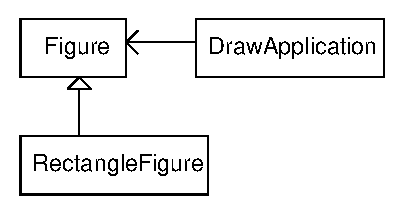
\includegraphics[width=0.4\textwidth]{class_samp.eps}
    \caption{例.クラス図.}
    \label{fig:class}
  \end{center}
\end{figure}

\section{プログラムの説明}
J3の場合は、作成したすべてのクラスの説明、クラス同士の関係、
実際に作成した各クラスの主な公開メソッド、公開フィールドの説明を行う。
必要に応じてプログラムリストを抜粋して説明する。

\section{実行例}
実行画面を示す.結果のみでなく,分かりやすく説明する.

必要に応じてグラフや図などを用いる.

例を 図\ref{fig:graph}に示す。

\begin{figure}[htbp]
  \begin{center}
    \leavevmode
    \includegraphics[width=0.6\textwidth]{graph.eps} 
% width=0.6\textwidth は図の横幅を全体の横幅の0.6倍に設定しています.
% 0.6 を変えると図の大きさを自由に変えることができます.
    \caption{例.sin(x)のグラフ.}
    \label{fig:graph}
  \end{center}
\end{figure}

課題J3の場合は、グラフの代わりにスクリーンショットをつけて、説明すること。

\section{考察}
実行結果に対する考察,コメント.

J3の場合は、実現したプログラムに対する考察、今後の改良点、
Javaや課題J3に付いての感想を述べよ。

\section{付録}
プログラムリストが2ページ以上になる場合は,本文中に含めないで,最後に
付録として付けるほうが読みやすい.

\verb|cat -n hash.c| などとして,行番号付きのプログラムリスト
を生成して,

\noindent
\verb|\begin{verbatim}....\end{verbatim}|を用いて記述すると読みやすい.
ページ数が多くなる場合は,
\verb|\small|や\verb|\footnotesize|を
用いるとよい.

\begin{small}
\begin{verbatim}
    1  struct item* insert(struct item s){
    2    int i; struct entry *p, *chain; 
    3    i=h(s.key);
    4    chain=H[i];
    5    if(chain){
    6      while(chain && comparekeytype(chain->term.key, s.key)) chain=chain->next; 
    7      if(chain) return &(chain->term);  /* 同じ鍵が見つかった 場合*/
    8    }

\end{verbatim}
\end{small}
\newpage
% 以下のチェックシートの()に○×もしくは1〜5の数値を入れ,必ず添付する
% こと.文章は変更しないこと.
\begin{Huge}
\begin{center}
{\bf レポート作成のためのチェックリスト\\
課題J3: Java\\}
提出前に○×を記入すること\\
\vskip 5mm

\ovalbox{
\begin{minipage}{0.98\textwidth}
\begin{list}{※}{\labelwidth=1.5zw}
\item 課題の目的と、実現すべきプログラムが何であるのかが
書かれているか? \hspace*{\fill} ( ) 
\item どのようにプログラムを設計しようとするのか,その設計方針につい
て書かれているか? \hspace*{\fill} ( ) 
\item 作成したプログラムの構成が(独立した文章で)分かりやすく書かれて
いるのか? \hspace*{\fill} ( ) 
\item 結果の検討や考察が明確に書かれているか? \hspace*{\fill} ( ) 
\item レポートの出来の自己評価は?\\
(最高を5とした5段階評価:     )
\end{list}
\end{minipage}
}
\end{center}
\end{Huge}
\end{document}
